
\documentclass[12pt, addpoints]{exam}
\usepackage[utf8]{inputenc}
\usepackage[portuguese]{babel}
\usepackage{multicol}
\usepackage{graphicx}
\usepackage{amsmath}
\usepackage{xcolor}
\usepackage[a4paper, portrait, margin=2cm]{geometry}

\setlength{\columnsep}{1cm}

        \begin{document}

        \begin{minipage}[l]{0.75\linewidth}
            \begin{flushleft}
                {\bf \Large Prova bimestral - LQ2N (2B)}
            \end{flushleft}
        \end{minipage}
        \begin{minipage}[r]{0.20\linewidth}
            \begin{flushright}
                {\bf \Large Código: 0}
            \end{flushright}
        \end{minipage}
        \vspace{0.5cm} \hrule \vspace{0.5cm}
        \begin{minipage}{0.75\linewidth}
            Aluno:
        \end{minipage}
        \begin{minipage}{0.20\linewidth}
            Data: 31/10/2022
        \end{minipage}
        \vspace{0.5cm} \hrule \vspace{0.5cm}
        \begin{center}
            \hqword{Question:}
            \hsword{Answer:}
            \cellwidth{2.2em}
            \gradetable[h][questions]
        \end{center}

        \begin{questions}
\begin{multicols*}{2}
\question[20] A figura abaixo mostra a trajetória de uma partícula carregada $\vec{v}$ representa a velocidade atravessando um campo magnético $\vec{B}$. Determine a sua trajetória devido a ação da força magnética atuando sobre ela.

\begin{center}
\begin{minipage}[c]{0.75\linewidth}
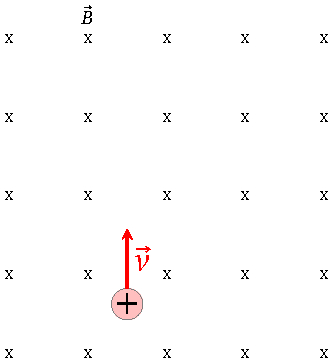
\includegraphics[width=\textwidth]{CEMAG001.jpg}
\end{minipage}
\end{center}
\begin{choices}
\choice Paralelo ao papel e circular no sentido horário.\choice Paralelo ao papel e da direita para a esquerda.\choice Paralelo ao papel e da esquerda para a direita.\choice Paralelo ao papel e na vertical.\choice Paralelo ao papel e circular no sentido anti-horário.\end{choices}
\question[20] Uma corrente elétrica de    5.91 percorre um fio de cobre. Sabendo-se que a carga de um elétron é igual a $1,6	imes 10^{-19}\;C$, qual é o número de elétrons que atravessa, por minuto, a seção reta desse fio?

\begin{oneparchoices}
\choice 1.61 \choice 2.34 \choice 3.78 \choice 3.93 \choice 4.5 \choice 9.08 \choice 5.4 \choice 1.78 \choice 5.91 \choice 2.45 \end{oneparchoices}
\end{multicols*}
\end{questions}
\newpage\end{document}